%% LaTeX-Beamer template for KIT design
%% by Erik Burger, Christian Hammer
%% title picture by Klaus Krogmann
%%
%% version 2.1
%%
%% mostly compatible to KIT corporate design v2.0
%% http://intranet.kit.edu/gestaltungsrichtlinien.php
%%
%% Problems, bugs and comments to
%% burger@kit.edu

\documentclass[18pt]{beamer}

%% SLIDE FORMAT

% use 'beamerthemekit' for standard 4:3 ratio
% for widescreen slides (16:9), use 'beamerthemekitwide'

\usepackage{templates/beamerthemekit}
\usepackage[utf8]{inputenc}
\usepackage[T1]{fontenc}
\usepackage{graphicx}
% \usepackage{templates/beamerthemekitwide}

%% TITLE PICTURE

% if a custom picture is to be used on the title page, copy it into the 'logos'
% directory, in the line below, replace 'mypicture' with the 
% filename (without extension) and uncomment the following line
% (picture proportions: 63 : 20 for standard, 169 : 40 for wide
% *.eps format if you use latex+dvips+ps2pdf, 
% *.jpg/*.png/*.pdf if you use pdflatex)

%\titleimage{mypicture}

%% TITLE LOGO

% for a custom logo on the front page, copy your file into the 'logos'
% directory, insert the filename in the line below and uncomment it

%\titlelogo{mylogo}

% (*.eps format if you use latex+dvips+ps2pdf,
% *.jpg/*.png/*.pdf if you use pdflatex)

%% TikZ INTEGRATION

% use these packages for PCM symbols and UML classes
% \usepackage{templates/tikzkit}
% \usepackage{templates/tikzuml}

% the presentation starts here

\title{Zwischenpräsentation der Java-Gruppe}
\subtitle{Neuronale Netze mit Neuroph}
\author{Markus Braun, Daniel Hammann, Dominik Messinger, Dominic Rausch}

\institute{Institut für Programmstrukturen und Datenorganisation (IPD), Lehrstuhl für Programmiersysteme}

% Bibliography

%\usepackage[citestyle=authoryear,bibstyle=numeric,hyperref,backend=biber]{biblatex}
%\addbibresource{templates/example.bib}
%\bibhang1em

\begin{document}
	\maketitle

	\begin{frame}[c]\frametitle{Neuronale Netze}
		\begin{block}{Einleitung}
		    \begin{itemize}
			    \item Bestehen aus Neuronen (Verarbeitungseinheiten)
		    	\item Gewichtete Eingabeverbindungen werden zusammenfasst (Propagierungsfunktion)
		    	\item Aktivierungsfunktion mit Schwellwert
		    	\item Aus Aktivierung folgt mittels Ausgabefunktion die Ausgabe
		    \end{itemize}		    
		\end{block}	
		\vspace{.5cm}
			\begin{minipage}[c]{0.48\textwidth}
				\begin{center}
				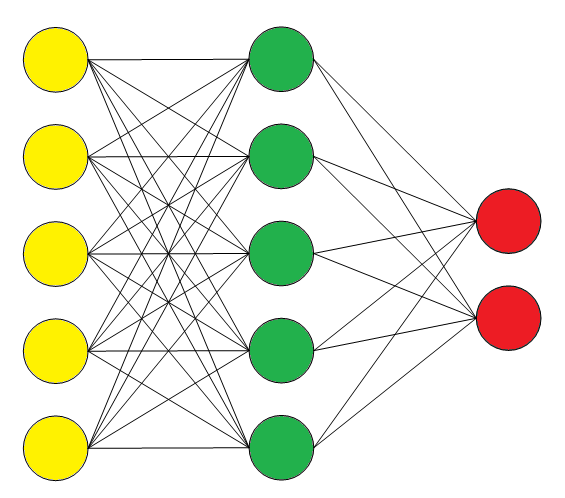
\includegraphics[width=0.5\textwidth]{images/ann.png}
				\end{center}
			\end{minipage}	
			\begin{minipage}[c]{0.48\textwidth}
				\begin{center}
				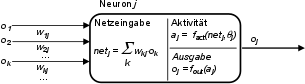
\includegraphics[width=\textwidth]{images/Neuron}
				\end{center}
			\end{minipage}
	\end{frame}
	
	\begin{frame}[c]\frametitle{Neuronale Netze}
		\begin{center}
		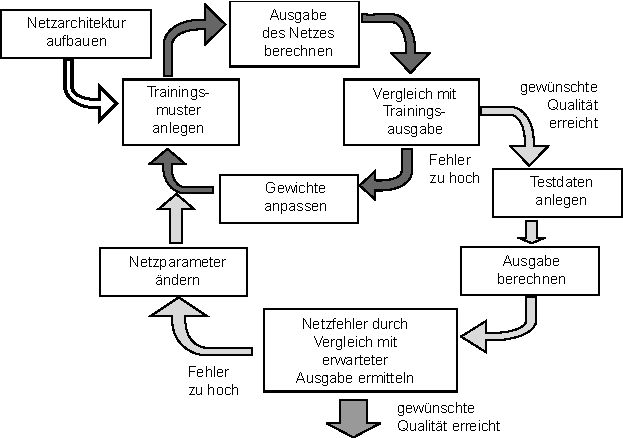
\includegraphics[scale=.8]{images/workflow}
		\end{center}
	\end{frame}		

	\begin{frame}[c]\frametitle{Überblick}
		\begin{block}{Was bisher geschah}
		    \begin{itemize}
		    	\item Einarbeitung in die Thematik der Neuronale Netze
			    \item Testdaten beschaffen
		    	\item Code Analyse der Simulationsumgebung Neuroph
		    	\item Drei Parallelisierungsversuche
		    	\item Profiling (u.a. eigenes Evaluierungsframework)
		    \end{itemize}		    
		\end{block}
	\end{frame}
	
	\begin{frame}[c]\frametitle{Testdaten}
		\begin{block}{Erste Versuche}
		    \begin{itemize}
		    	\item StockExchange - Börsenvorhersage
		    	\item IrisScan Datensatz
		    \end{itemize}
		\end{block}
		\begin{block}{Teilchenkollision (Cern)}
		    \begin{itemize}
		    	\item 15k Datensätze
		    	\item Eingabe: 2853 Sensorwerte
				\item Ausgabe: Ist das Ereignis interessant oder nicht? 
				%Schwarzes Loch oder nicht?
		    \end{itemize}
		\end{block}		
	\end{frame}

	\begin{frame}[c]\frametitle{Code Analyse \& Profiling}
		\begin{block}{Was wir vorgefunden haben}
			\begin{center}
				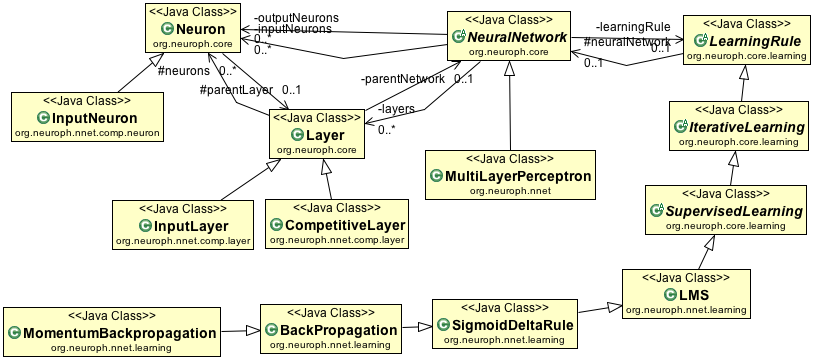
\includegraphics[scale=0.4]{images/Klassendiagramm.png}
			\end{center}
		\end{block}
	\end{frame}
	
	\begin{frame}[c]\frametitle{Code Analyse \& Profiling}
		\begin{block}{Sequenzdiagramm}
			\begin{center}
			  %\textit{TODO: Sequenzdiagramm} 
			  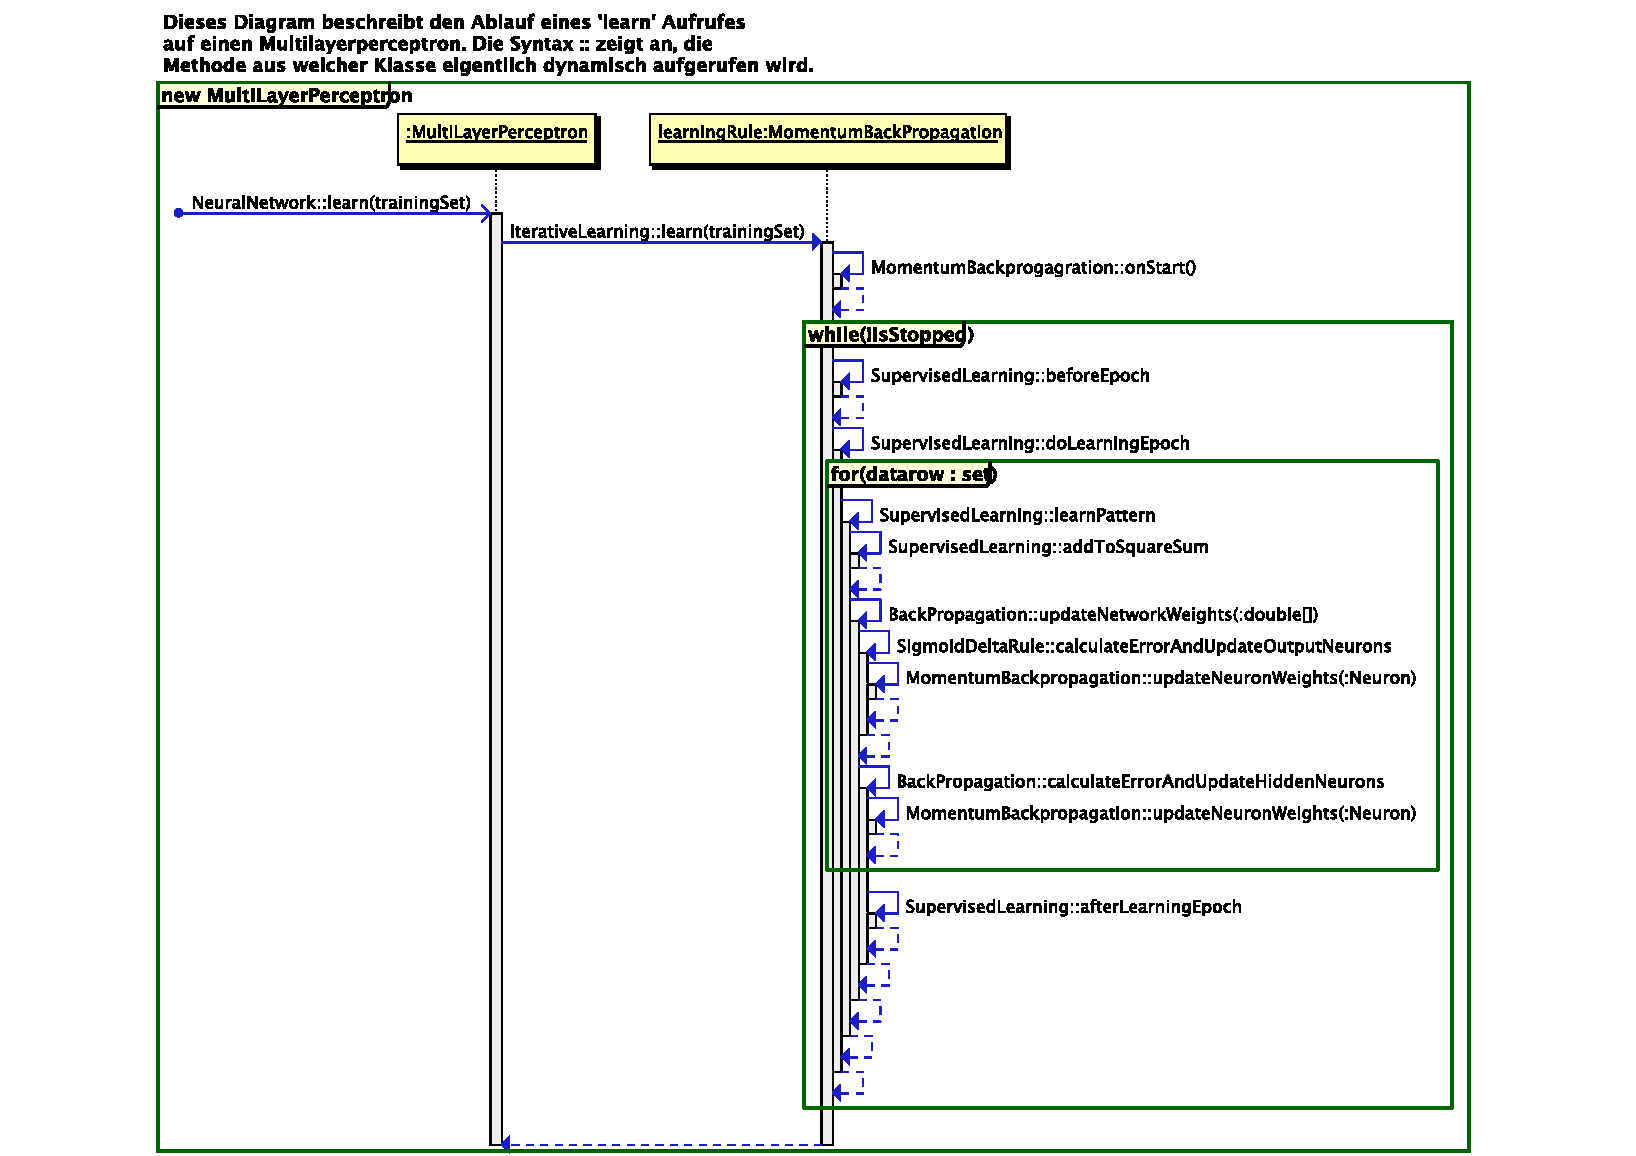
\includegraphics[scale=0.3]{images/Learn.pdf} 
			\end{center}
		\end{block}
	\end {frame}
	
	\begin{frame}[c]\frametitle{Code Analyse \& Profiling}
		\begin{block}{Profiling}
			Methoden mit höchster akkumulierter Rechenzeit:
			\begin{itemize}
				\item $Connection.getInput()$
				\item $Connection.getWeightedInput()$
		    \end{itemize}
			$\rightarrow$ Zeit korreliert mit Anzahl der $Connections$ und Anzahl der Lern-Iterationen
		\end{block}
	\end {frame}			
	
	\begin{frame}[c]\frametitle{Parallelisierungsansätze}
		%\begin{alertblock}{}
		%\textit{TODO: Hier alle Unterpunkte rausnehmen (auf nachfolgende Seiten verteilen) und nur als kurze Übersichtsfolie nutzen??} Ja.
		%\end{alertblock}
		\begin{itemize}
			\item Layer-Partitionierung
			%\begin{itemize}
				%\item Mehrere Neuronen einer Schicht pro Thread
				%\item Langsam, da zu fein granular
			%\end{itemize}
			\item Batch Learning Parallelisierung
			%\begin{itemize}
				%\item Batch parallelisieren
				%\item Einfacherer zu parallelisieren
			%\end{itemize}
			\item Clonebased Parallelisierung
			%\begin{itemize}
				%\item Ergebnis entspricht nicht dem Orginal
				%\item Lernen bleibt unmodifiziert 
			%\end{itemize}
		\end{itemize}	
	\end{frame}
	
	\begin{frame}[c]\frametitle{Layer-Partitionierung}
		\begin{itemize}
			\item Ansatz:
			 \begin{itemize}
				\item Parallel Auswertung innerhalb partitionierter Neuronenschichten
			\end{itemize}
			\item Evaluation:
			\begin{itemize}
				\item Zu feingranular, Concurrency-Overhead überwiegt erhoffte Zeitersparnis
			\end{itemize}
		\end{itemize}	
	\end{frame}

	\begin{frame}[c]\frametitle{Batch Learning Parallelisierung}
		\begin{itemize}
			\item Batch Learning
			\begin{itemize}
				\item Summieren der Deltas (pro Verbindung)
				\item Aktualisieren erst nach einer Epoche
			\end{itemize}
			\item Ablauf:
			\begin{itemize}
				\item Aufteilen der Lerndaten
				\item Jeder Thread summiert Deltas
				\item Aktualisieren der Gewichte
			\end{itemize}
			\item Klone des NN notwendig
		\end{itemize}
	\end{frame}
	
	\begin{frame}\frametitle{Batch Learning Parallelisierung}
		\begin{enumerate}
			\item NN klonen (tiefe Kopie)
			\item Daten aufteilen
			\item \textit{parallel:} Jeder Thread lernt seine Daten
			\item \textit{parallel:} Gewichte der Klone in das Hautp-NN mergen (und in die Klone)
			\item \textit{Barriere}n
			\item Fehlerberechnung
			\item Fehler < x ? Fertig : Goto 3
		\end{enumerate}
	\end{frame}
	
	\begin{frame}\frametitle{Clonebased Parallelisierung}
		\begin{center}
			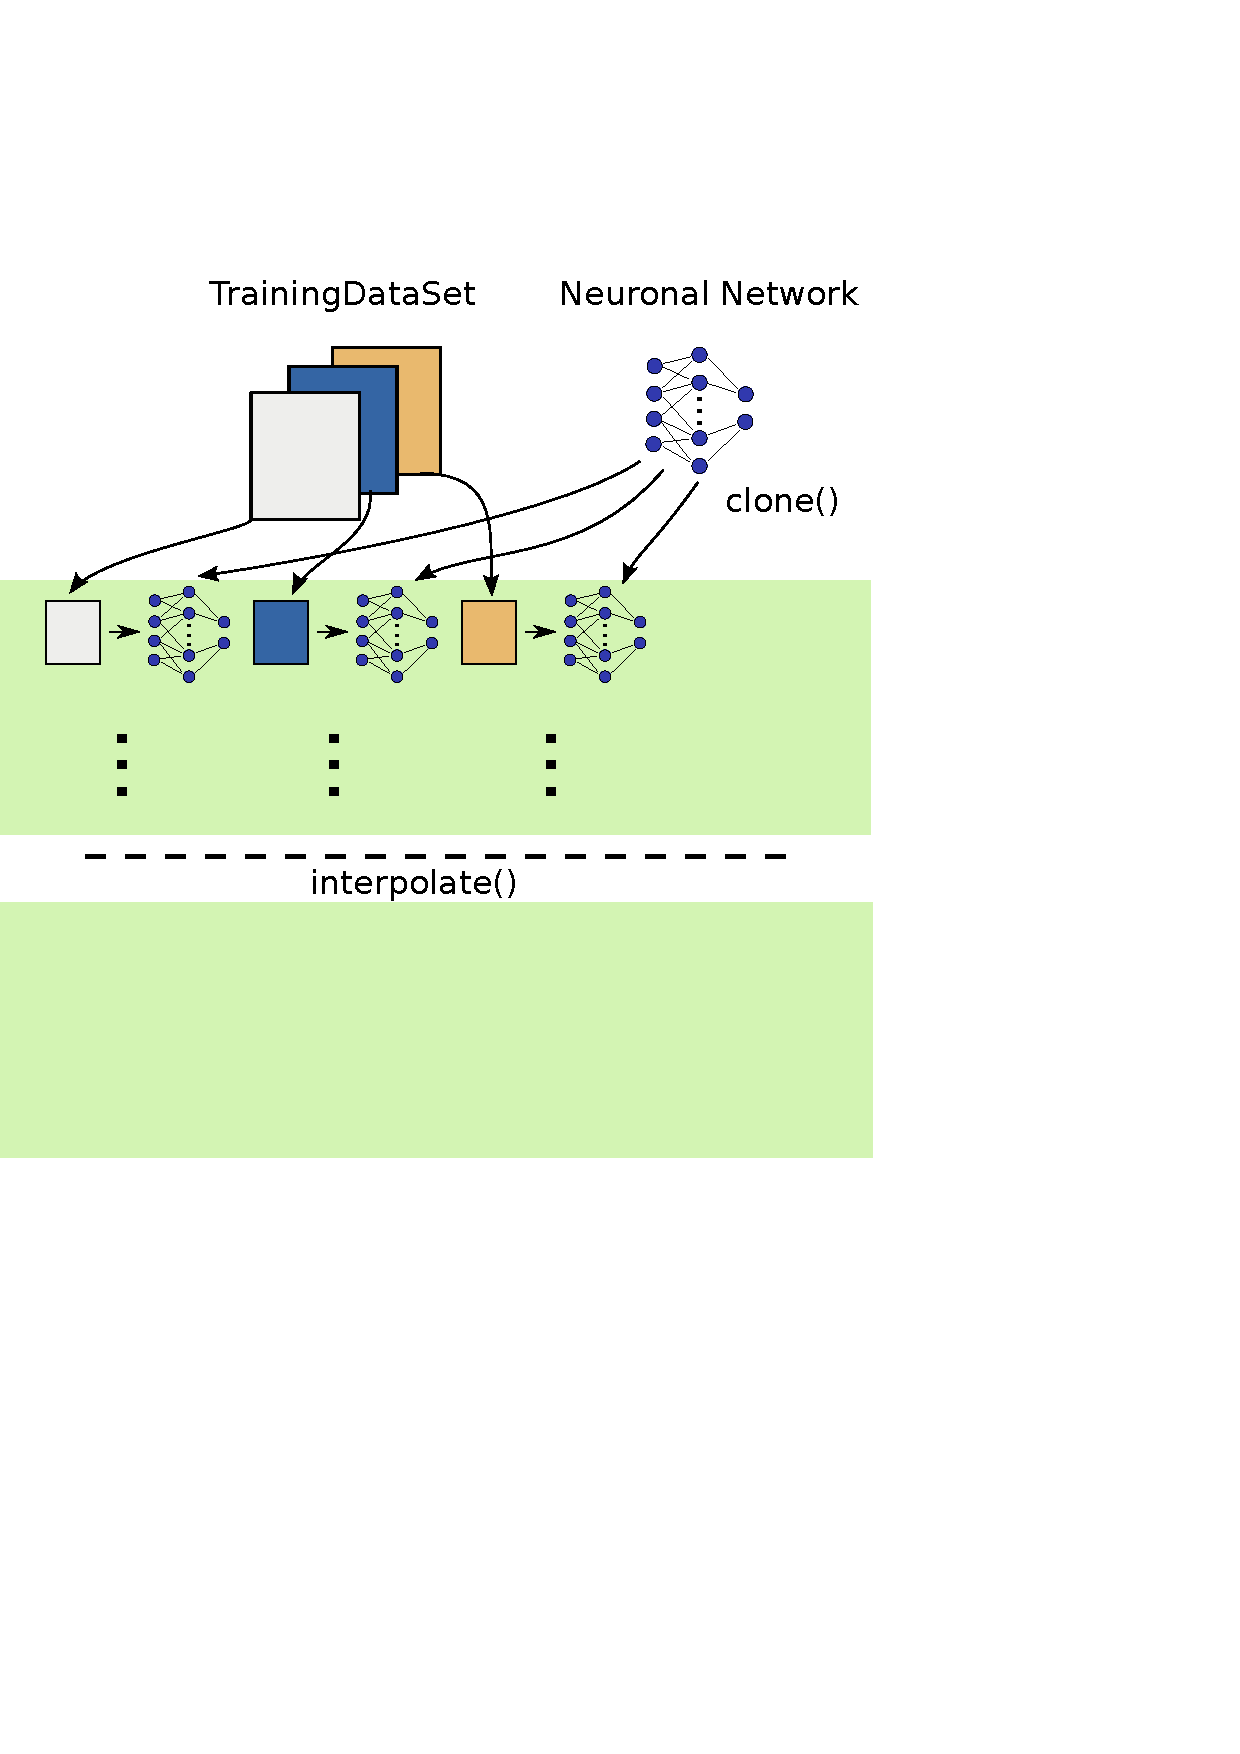
\includegraphics[width=.65\textwidth]{images/Parallelisierungsansatz.pdf} 
		\end{center}
	\end{frame}
	
	\begin{frame}\frametitle{Clonebased Parallelisierung}
		\begin{itemize}
			\item ANN wird nach der Erzeugung \glqq geklont\grqq
			\item Ein Klon pro Thread
			\item Unterschiedliche Interpolationsfunktionen
			\item Weitere Parameter
			\begin{itemize}
				\item Synchronisationsintervall
				\item Maximale Anzahl von Iterationen
			\end{itemize}				
			\item Andere Ergebnisgewichte als bei sequentiellem Lernen
			\item Wrapper für ein neuronales Netz
		\end{itemize}
	\end{frame}


	%  TODO: Dominik Clone worker parallelisierung...


%TODO: Evaluierung, Zwischenstand, Erwähnen, dass Güte über Zeit und Fehler gemessen wird. Exakt gleich Ergebnis ist nicht erforderlich. Evaluierungsframework

	\begin{frame}\frametitle{Evaluationsframework}
		\begin{block}{Score}
			wird bestimmt durch
		    \begin{itemize}
		    	\item Fehler (auf Testdaten)
		    	\item Laufzeit
		    \end{itemize}
		\end{block}
		\begin{block}{Vorgehen}
		    \begin{enumerate}
		    	\item Permutation der Daten
		    	\item Aufteilung in Trainings- und Testdaten
				\item $foreach$ ILearner L $do$
				\begin{itemize}
					\item Lerne Trainingsdaten und messe Ausführungszeiten
					\item Berechne Fehler auf Testdaten
				\end{itemize}
				\item Wiederhole ab 1 bis gewünschte Anzahl an Läufen erreicht
		    \end{enumerate}
		\end{block}
	\end{frame}

	\begin{frame}\frametitle{Whats next?}
		\begin{block}{Fahrplan}
		    \begin{itemize}
		    	\item Vollständige Evaluierung der Ansätze
		    	\item Experimentieren mit unterschiedlichen Konfigurationsparametern $\rightarrow$ Speedup
		    \end{itemize}
		\end{block}
	\end{frame}

\end{document}